\chapter{วิธีการดำเนินการวิจัย}
\label{chapter:experiment}

ในส่วนของบทนี้จะพูดถึงลักษณะต่าง ๆ ของข้อมูลเสียงที่ได้ การดำเนินงานในการจัดการกับข้อมูลเสียง 
และสร้างแบบจำลองในแบบต่าง ๆ เพื่อคาดคะเนสายพันธุ์ของนกออกมาเป็นแบบหลายๆฉลาก (multi-label classification) 
ซึ่งลักษณะของข้อมูลเสียงที่ถูกนำมาใช้ในการทดลองและผลงานวิจัยที่เกี่ยวข้องจะถูกพูดถึงในหัวข้อที่ 3.1 
ขั้นตอนการดำเนินงานทั้งหมดจะถูกกล่าวถึงในหัวข้อที่ 3.2 จนถึง หัวข้อที่ 3.4 และจะมีการสรุปผลการศึกษางานวิจัยที่เกี่ยวข้องและ
ขั้นตอนการดำเนินงานทั้งหมดในหัวข้อที่ 3.5

\section{บทนำและงานวิจัยที่เกี่ยวข้อง}
\subsection{การเก็บข้อมูลและลักษณะของข้อมูลเสียง ที่ถูกนำมาใช้ในการทดลอง}
ข้อมูลในส่วนที่ถูกนำมาใช้ ให้เป็นข้อมูลสำหรับการฝึกในครั้งนี้ คือข้อมูลที่มาจากการแข่งขันในปี ค.ศ. 2019~\cite{Kahl2019} แต่ถูกปรับเปลี่ยน 
และพัฒนาคุณภาพขึ้นมาใหม่โดยผู้จัดหาและจัดทำข้อมูลรายใหม่อย่าง Xeno-canto~\cite{xeno-canto}ที่เป็นเว็บไซต์ให้ผู้คนในสาขาต่างๆ ได้ร่วมกันแบ่งปันข้อมูลเสียงนกจากทุกที่ทั่วโลก 
และตัวเว็บไซต์เองไม่ได้เป็นแค่ชุดสะสมการบันทึกเสียงนกเพียงเท่านั้น แต่ยังเป็นโครงงานความร่วมมือที่พร้อมจะให้ทุกคนที่ใช้งานเว็บไซต์มีส่วนร่วมในการช่วยกันแบ่งปันเสียงบันทึกของนก 
และระบุเสียงของนกชนิดต่างๆที่ปรากฏอยู่บนเว็บไซต์ด้วย \par

ข้อมูลจากการแข่งขันเมื่อปี ค.ศ. 2019 นั้น ประกอบไปด้วยทัศนียภาพของเสียงที่ถูกบันทึกด้วยมือกว่า 350 ชั่วโมง ซึ่งโดยส่วนใหญ่ถูกบันทึกไว้ด้วยเครื่องอัดเสียงภาคสนาม 
ช่วงเดือน มกราคม และเดือนมิถุนายน ในปี ค.ศ. 2017 ที่เมืองอิทากา นครนิวยอร์ก ประเทศสหรัฐอเมริกา (Ithaca, NY, USA) และใช้เครื่องบันทึกเสียงรอบทิศทางที่ถูกจัดหาไว้โดยโครงการวิจัยด้านชีวเคมี 
ประจำห้องปฏิบัติการด้านปักษีวิทยา แห่งมหาวิทยาลัยคอร์เนล (Bioacoustics Research Program of the Cornell Lab of Ornithology) 
เครื่องบันทึกเสียงเหล่านี้ สามารถบันทึกเสียงได้มากกว่า 30 หน่วยที่ขยายไปทั้งหมด 1 ตารางไมล์ผ่านแหล่งน้ำที่หลากหลาย และพืชพรรณหลายๆชนิด ซึ่งผู้ติดตั้งและผู้จัดการข้อมูลได้สุ่มเลือก 1 ไฟล์สำหรับแต่ละชั่วโมงในหนึ่งวัน ที่ถูกบันทึกจากเครื่องบันทึก 1 
ใน 30 ตัวที่ถูกติดตั้งไว้ มารวบรวมและบันทึกไฟล์เข้าไว้ด้วยกันเป็นจำนวนทั้งหมด 15 วัน หลังจากนั้นก็นำไฟล์เสียงที่บันทึกไว้มาให้ผู้เชี่ยวชาญ อธิบายและทำเครื่องหมายไว้ว่าแต่ละช่วงเวลาในไฟล์ที่ถูกแบ่งไว้เป็นช่วงๆ ช่วงละ 5 วินาทีนั้น เป็นของนกสายพันธุ์ไหน \par

นอกจากนี้ในตัวชุดข้อมูลเมื่อปี ค.ศ. 2019 ได้มีการหยิบชุดข้อมูลจากการแข่งขัน BirdCLEF เมื่อปี ค.ศ. 2018 กลับมาใช้ซ้ำด้วย ซึ่งเป็นข้อมูลทัศนียภาพของเสียงที่มีความยาวทั้งหมดอยู่ประมาณ 4 ถึง 5 ชั่วโมง ซึ่งข้อมูลดังกล่าวถูกบันทึกที่ประเทศโคลอมเบีย 
โดยนักปักษีวิทยาจากมูลนิธิความหลากหลายทางชีวภาพแห่งโคลอมเบีย ที่มีชื่อว่า Paula Caycedo Rosales และสมาชิกของ Xeno-canto สามารถดูรายละเอียดเกี่ยวกับทัศนียภาพของเสียงโดยรวมได้ที่ หมายเหตุการทำงานของการแข่งขัน BirdCLEF เมื่อปี ค.ศ. 2018~\cite{Goeau2018} \par

ข้อมูลที่ใช้ในการฝึกแบบจำลอง สำหรับการแข่งขัน BirdCLEF ในปีนี้จะประกอบไปด้วยเสียงบันทึกของนกสายพันธุ์ต่างๆที่มาจากทั้งอเมริกาเหนือ อเมริกาใต้ และโซนยุโรป โดยที่ชุมชนของเว็บไซต์ Xeno-canto เป็นผู้จัดหาและสนับสนุนชุดข้อมูลการบันทึกเสียงคุณภาพสูงกว่า 
70,000 การบันทึก ผ่านทางสายพันธุ์นกทั้งหมดกว่า 960 สายพันธุ์ การบันทึกในแต่ละครั้งจะมีเมตาดาต้า (metadata) ประกอบไปกับการบันทึกด้วย โดยในเทตาดาต้าจะประกอบไปด้วย 
สถานที่ในการเก็บบันทึก เวลา และคำอธิบายอื่นๆที่ถูกจัดไว้ให้โดยผู้บันทึกเสียงในการบันทึกครั้งนั้นๆ \par


ส่วนข้อมูลที่จะถูกนำไปใช้ในการทดสอบแบบจำลอง จะประกอบไปทัศนียภาพของเสียงโดยรอบกว่า 153 เสียงที่ถูกบันทึกไว้ในประเทศเปรู สหรัฐอเมริกา และประเทศเยอรมนี โดยในแต่ละเสียงที่ปรากฏ 
จะมีระยะเวลาทั้งหมด 10 นาทีและมีการเปล่งเสียงของนกที่ทับซ้อนกันภายในแต่ละช่วงเวลาในปริมาณที่ค่อนข้างสูง

\subsection{พฤติกรรมการส่งเสียงร้องของนก}
นกใช้เวลาส่วนใหญ่ไปกับการส่งเสียงร้อง แต่ในขณะเดียวกันเสียงร้องของนกในแต่ฤดูกาลจะมีความแตกต่างกัน วัตถุประสงค์ในการส่งเสียงร้องของนกแบ่งออกเป็น 2 อย่างหลัก ๆ ประการแรกคือ นกเพศผู้จะส่งเสียงร้องเพื่อบ่งบอกถึงอาณาเขตของตนเอง 
และประกาศให้ศัตรูรับรู้ว่าจะปกป้องอาณาเขตของตนเองจากเผ่าพันธุ์อื่น ส่วนวัตถุประสงค์ที่สองคือ นกจะส่งเสียงร้องเพื่อดึงดูดคู่ครองและสร้างรัง นกเพศเมียมักจะเลือกคู่ครองโดยขึ้นอยู่กับการผสมผสานระหว่างการมองเห็นและเสียงร้อง 
แม้แต่นกเพศผู้ที่มีขนที่สวยงามในฤดูผสมพันธ์ ก็มีปัญหาในการหาคู่ครองเนื่องจากเสียงร้องที่ไม่สามารถเข้ากันได้ นกแต่ละสายพันธุ์จะมีเสียงร้องเป็นเอกลักษณ์ของตัวเอง 
ทำให้เมื่อนกได้ยินเสียงร้องจะสามารถแยกได้ว่าเสียงร้องนั้นมาจากสายพันธุ์ของตนเองหรือไม่ ถึงแม้ว่านกจะใช้เวลาและพลังงานส่วนใหญ่ไปกับการส่งเสียงร้อง แต่ก็ไม่สามารถทำได้ตลอดทุกฤดูกาล 
โดยส่วนใหญ่จะส่งเสียงร้องมากที่สุดในระหว่างฤดูการทำรังและเมื่อฤดูทำรังสิ้นสุดลงนกจะส่งเสียงร้องน้อยลงและอาณาเขตของพวกมันจะพังทลายลงเนื่องจากมีนกหลายชนิดที่จะทำการอพยพตามฤดูกาล ในนกหลายสายพันธุ์จะมีเพียงเพศผู้ที่ส่งเสียงร้องเท่านั้น 
แต่นอกเหนือจากนั้นนกจะส่งเสียงร้องทั้งเพศผู้และเพศเมีย และในนกบางตัวจะไม่มีการส่งเสียงเลย เช่นอีแร้งและนกกระสาที่แทบจะไม่สามารถสร้างเสียงใด ๆได้~\cite{EarthSky}
ในการระบุสายพันธุ์ของนกด้วยเสียงร้องสามารถสังเกตุได้จากคุณลักษณะของเสียงร้องที่แตกต่างกัน 7 คุณลักษณะ~\cite{Birdingbyear} ดังต่อไปนี้ 

\begin{itemize}
    \item \textbf{ระดับเสียง (Pitch)} เสียงร้องมีความสูงหรือต่ำแค่ไหน?
    \item \textbf{คุณภาพของเสียง (Quality)} มีเสียงที่แตกต่างกันในเสียงร้องหรือไม่? 
    \item \textbf{ความยาว (Length)} เสียงร้องมีความยาวเท่าไหร่? ใช้เวลาเท่าไหร่ในการร้องซ้ำ
    \item \textbf{ความเร็วเพลง (Tempo)} เสียงร้องมีกี่จังหวะ เร็วแค่ไหน? หรือช่วงไหนของเสียงร้องมีการหยุดชั่วคราว
    \item \textbf{ความดังของเสียง (Volume)} เสียงร้องมีการเปลี่ยนระดับความดังหรือไม่? ถ้ามีการเปลี่ยนระดับความดังของเสียง เปลี่ยนที่ตำแหน่งใดและเปลี่ยนอย่างไร? นกที่มีเสียงร้องคล้ายกันแต่ต่างชนิดกันจะมีความดังของเสียงที่ต่างกัน
    \item \textbf{การทำซ้ำ (Repetition)} มีพยางค์ของเสียงที่เหมือนกันซ้ำกันหลายครั้งหรือไม่ ซ้ำกันกี่ครั้ง และมีลำดับที่คล้ายกันเป็นส่วนหนึ่งของเสียงร้องเท่าไหร่?
    \item \textbf{การจำลอง (Mimicry)} มีเสียงที่ผิดปกติที่คล้ายสิ่งอื่นในเสียงร้องหรือไม่ เช่น เสียงสัญญาณกันขโมย เสียงเครื่องมือต่าง ๆ เนื่องจากอาจมีการเลียนแบบเสียงร้องของนก
\end{itemize}

\subsection{กระบวนการขั้นพื้นฐาน (Baseline methods)}
วิธีพื้นฐานที่ใช้กันทั่วไปในการสืบค้นเสียงมีพื้นฐานมาจากพลังงานอย่างใดอย่างหนึ่ง ไม่ว่าจะเป็นคลื่นสเปคตรัมข้ามสหสัมพันธ์ (spectrogram cross-correlation) แบบจำลองมาร์คอฟซ่อนเร้น (Hidden Markov model (HMM))~\cite{Yoon2009} ซึ่งกระบวนการพื้นฐานที่กล่าวมานี้มักเป็นที่รู้จักและ
ใช้กันทั่วไปในการทำวิจัยเกี่ยวกับเสียงสะท้อนชีวภาพ (bioacoustics) \par
แต่ในบางครั้งวิธีที่ง่ายที่สุดมักเป็นการตั้งค่าจุดเปลี่ยนผ่านหากค่าผลลัพธ์ที่ได้ มีค่าสูงกว่าค่าที่ตั้งไว้ (thresholding) ซึ่งจะมีผลลัพธ์เป็นบวก (positive) หากค่าพลังงานในช่วงเวลาสั้นๆที่ตัดมานั้นมีค่าสูงกว่าค่าที่ตั้งไว้
และนอกจากนั้นจะเป็นค่าลบ (negative) และสำหรับการทำเสียงสะท้อนชีวภาพมักจะมีการจัดการกับเสียงรบกวน และการเพิ่มชุดข้อมูล (data augmentation) เพื่อประมาณค่าของเสียงรบกวนที่ได้มาเมื่อเวลาผ่านไป 
และเพื่อให้มั่นใจว่าสามารถรับมือกับเสียงรบกวนได้ตลอด \par
นอกเหนือจากนี้แล้วการจัดแข่ง BirdClef ประจำปีค.ศ. 2018 ได้ให้ตัวอย่างลำดับการทำงานคร่าว ๆ ในการจัดการกับเสียงนกที่ใช้ในการแข่งขันมาเป็นระบบในการตรวจจับเสียงนกแบบพื้นฐาน (Baseline system)~\cite{Kahl2018}
เพื่อให้ผู้เข้าแข่งขันสามารถนำระบบพื้นฐานที่ได้ไปพัฒนาระบบขึ้นมาใหม่เพื่อให้ได้ผลลัพธ์ที่ดีขึ้น โดยระบบพื้นฐานในการตรวจจับเสียงนกที่ผู้จัดแข่งขันให้มานั้นได้ระบุถึงลำดับการทำงาน (Workflow) รายละเอียดชุดข้อมูลสถาปัตยกรรมโครงข่ายประสาทแบบคอนโวลูชัน (CNN Architecture)
การประเมินผล และแนวทางในการพัฒนาระบบต่อไปด้วย

\section{การจัดเตรียมการทดลอง}
ข้อมูลที่ได้จากการแข่งขันในรอบปี ค.ศ. 2020 นี้ได้แบ่งไว้เป็นข้อมูล 3 ชุดหลักๆคือ ข้อมูลที่ใช้สำหรับการฝึกแบบจำลอง (training data) ข้อมูลที่ใช้สำหรับการทดสอบประสิทธิภาพของแบบจำลองเพื่อหา Hyperparameter ที่ดีที่สุด (validation data) และข้อมูลที่ไว้ใช้สำหรับการทดสอบแบบจำลอง (test data) ซึ่งก่อนที่จะสามารถสร้างแบบจำลอง
หรือทำนายผลออกมาได้อย่างสมบูรณ์ก็ต้องมีการ ทำความเข้าใจตัวชุดข้อมูล และจัดเตรียมข้อมูลก่อนนำข้อมูลเข้าให้ดีก่อน
\subsection{การสำรวจชุดข้อมูลเสียงนก (Data exploration)}
จาการสำรวจข้อมูลในเบื้องต้นพบว่าข้อมูลถูกแบ่งออกเป็น 3 ส่วนใหญ่ ๆ โดยมีลายละเอียดดังต่อไปนี้

\begin{itemize}
    \item \textbf{Audio Training Set} ข้อมูลชุดข้อมูลนี้เป็นชุดข้อมูลที่ความไม่สมดุลกันของข้อมูลและข้อมูลชุดนี้ประกอบไปด้วยไฟล์เสียงของนกทั้งหมด 961 สายพันธุ์โดยมีไฟล์เสียงนกทั้งหมด 72324 ไฟล์โดยจัดเก็บนกแต่ละสายพันธุ์ไว้ด้วยโฟลเดอร์ดังที่แสดงในรูป \ref{Fig:folder} และเก็บไฟล์เสียงของนกแต่ละสายพันธุ์จะถูกจัดเก็บไว้ในโฟลเดอร์ที่เก็บไฟล์ .mp3 หลายๆไฟล์ดังที่แสดงในรูป \ref{Fig:filemp3}
    \begin{figure}[h]
        \centering
        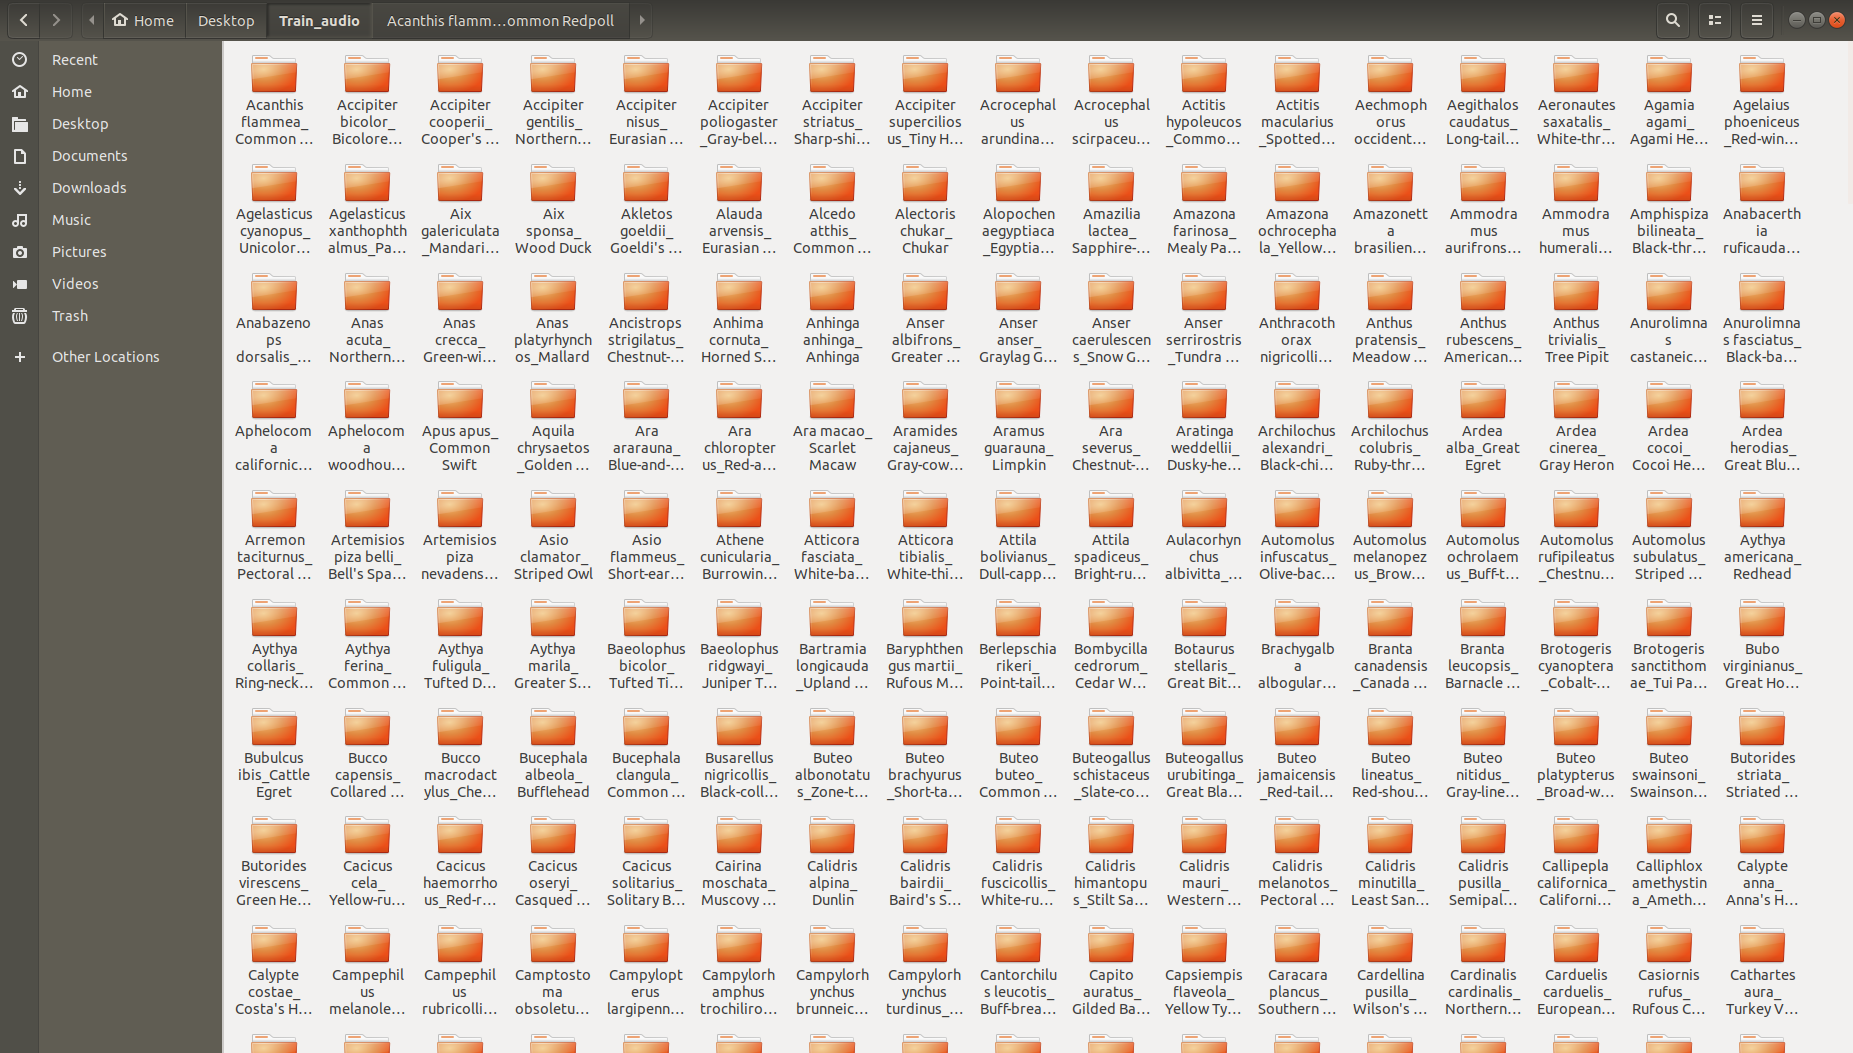
\includegraphics[scale = 0.15]{folder.png}
        \caption{โฟล์เดอร์ที่ใช้ในการเก็บไฟล์เสียง}
        \label{Fig:folder}
    \end{figure}
    \begin{figure}[h]
        \centering
        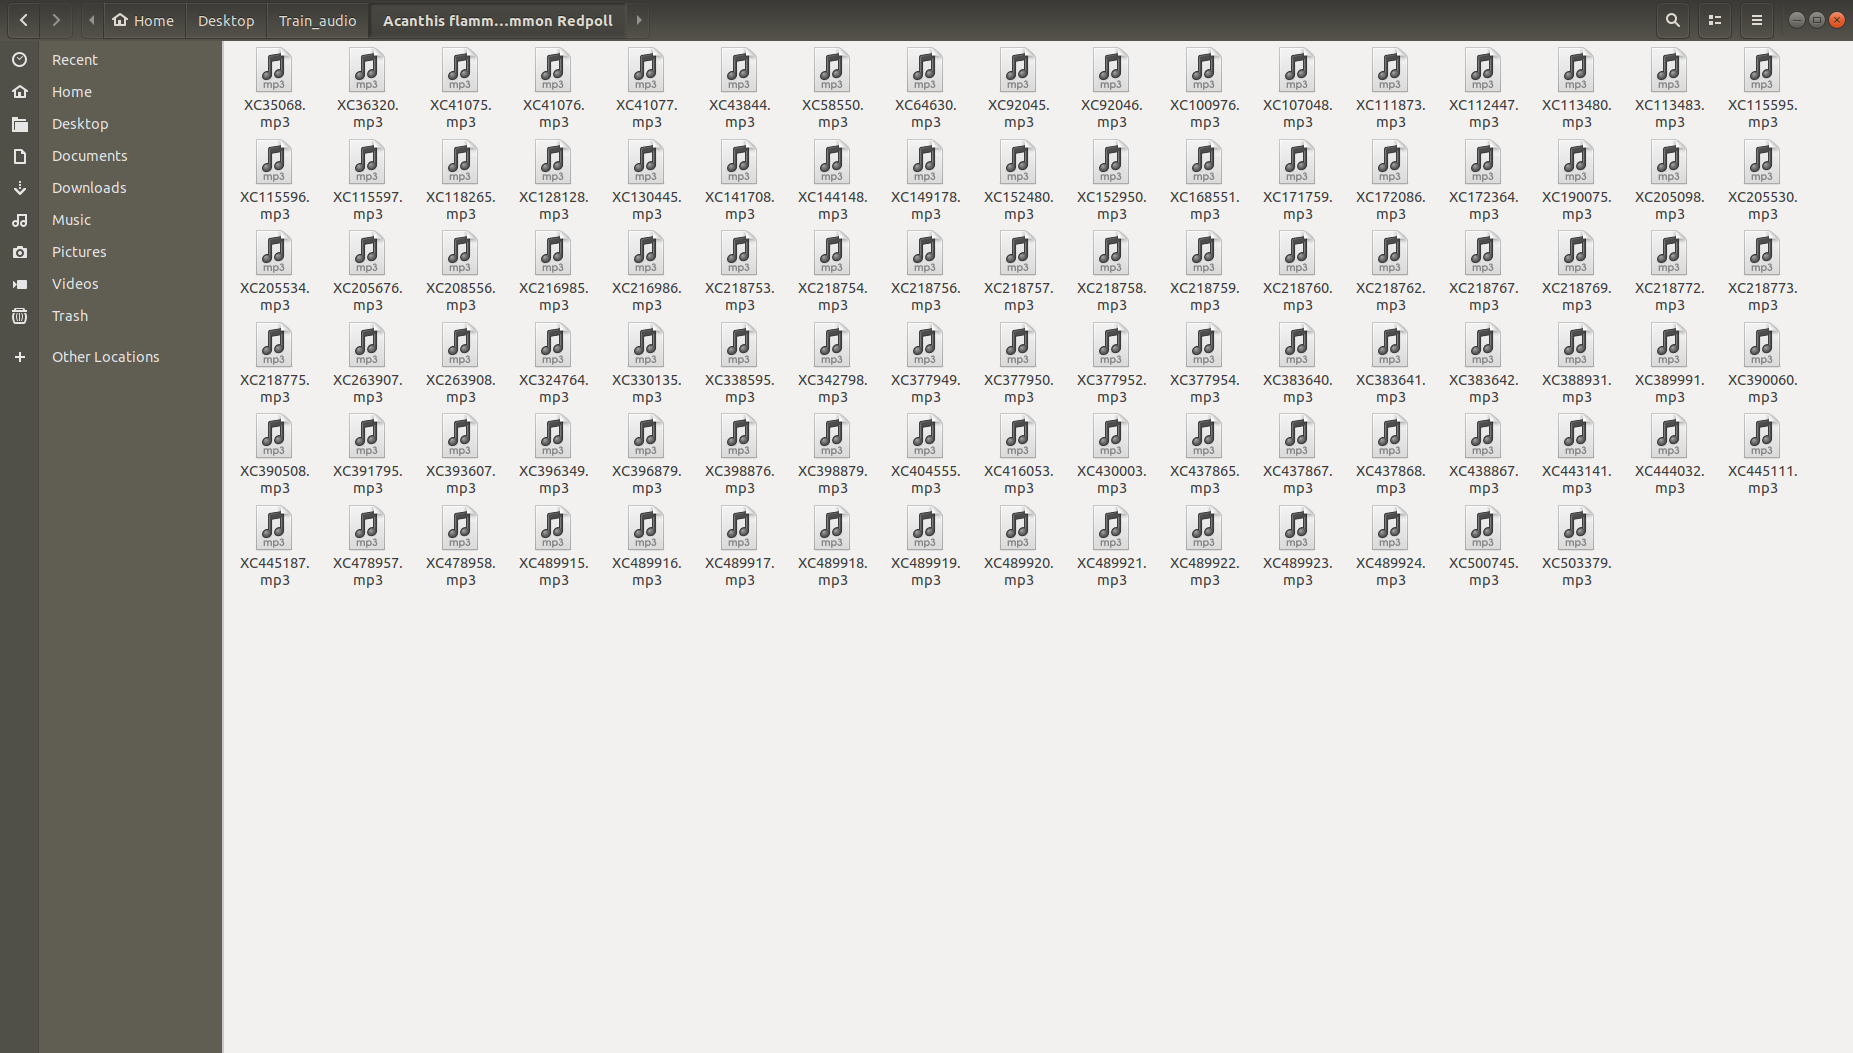
\includegraphics[scale = 0.15]{filemp3.png}
        \caption{ตัวอย่างไฟล์เสียงที่ถูกเก็บไว้ในโฟร์เดอร์}
        \label{Fig:filemp3}
    \end{figure}
    \FloatBarrier

    \item \textbf{Audio Validation set} ข้อมูลชุดนี้คือข้อมูลที่ใช้ในการทดสอบแบบจำลองเพื่อหาค่า Hyperparameter ที่ดีที่สุด โดยข้อมูลในชุดนี้ประกอบไปด้วยข้อมูลเสียงที่เป็นไฟล์ .wav ทั้งหมด 12 ไฟล์ ซึ่งไฟล์เหล่านี้จะถูกนำเข้าไปประมวลผลในแบบจำลองและทำนายว่าเสียงของนก ณ ช่วงเวลานั้น 
    เป็นเสียงของนกสายพันธุ์ใด และอีกส่วนคือไฟล์ข้อมูลที่เป็นไฟล์ .csv ซึ่งทั้งหมด 12 ไฟล์ซึ่งเป็นไฟล์เฉลยสำหรับการทำนายที่ได้จากแบบจำลอง ดังที่แสดงในรูป \ref{Fig:validate} โดยในช่องแรกจะเป็นช่องที่แสดงถึงช่วงเวลาของที่อยู่ภายในไฟล์เสียงนั้นๆ และช่องที่สองคือช่องที่บอกว่าในแต่ละช่วงเวลานั้นเสียงที่ได้ยินคือเสียงของนกสายพันธุ์อะไรแล้วจึงนำค่าที่ได้จากการทดสอบแบบจำลองไปปรับเปลี่ยนการตั้งค่า และหาค่า Hyperparameter ใหม่ให้กับแบบจำลองตามความเหมาะสม
    \item \textbf{Audio Test set} คือชุดข้อมูลที่ไว้ใช้สำหรับทดสอบแบบจำลองที่ประกอบไปด้วยไฟล์เสียง .wav รวมอยู่ทั้งหมด 153 ไฟล์ที่เป็นไฟล์ทัศนียภาพของเสียง โดยแต่ละไฟล์จะมีความยาวอยู่ที่ไฟล์ละ 10 นาที ซึ่งเราต้องนำแบบจำลองของเราไปประมวลผลผ่านไฟล์ที่ได้เพื่อให้ได้คำตอบออกมาดังรูปที่ \ref{Fig:validate} และนำไฟล์คำตอบเหล่านั้นส่งไปยังเว็บไซต์ [21] ที่ผู้จัดแข่ง BirdCLEF 2020 เป็นคนกำหนด
    \begin{figure}[h]
        \centering
        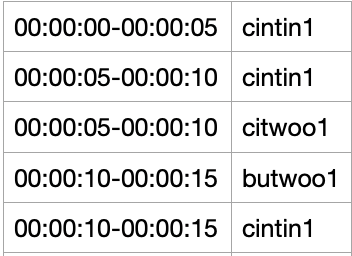
\includegraphics[scale = 0.7]{validation.png}
        \caption{ไฟล์เฉลยการทำงานของแบบจำลอง}
        \label{Fig:validate}
    \end{figure}
    \FloatBarrier
\end{itemize}




% จากกราฟสามารถสรุปชื่อและจำนวนที่พบของนก 6 
% สายพันธุ์ที่พบมากที่สุดในชุดข้อมูลทดสอบประสิทธิภาพของแบบจำลองได้ดังตารางที่ 3.1

% \begin{table}[ht]
%     \centering
%     \caption{แสดงชื่อและจำนวนของนกที่พบมากที่สุด 6 สายพันธุ์}
    
%     \begin{tabular}{|l|c|c|} \hline
%     \multicolumn{1}{|c|}{ชื่อสายพันธ์ุ} & รหัสสายพันธุ์ & จำนวนที่พบ \\ \hline
%     Turdus hauxwelli\_Hauxwell's Thrush   & hauthr1 & 218 \\  \hline
        
%     \end{tabular}
% \end{table}

\subsection{Metrics ที่ใช้สำหรับการประเมินประสิทธิภาพของแบบจำลอง}
